\chapter{Integrales de trayectoria	 en espacio plano.}
El formalismo mas común de la mecánica cuantica se deriva de cambiar las variables clasicas de posición y momentum ($p$ y $q$) por operadores que obedecen el álgebra:
\begin{equation}
[\hat{q},\hat{p}]=i\hbar
\end{equation}
Esta relación se conoce como la condción de cuantización de Heisenberg, en general en la mecánica cuantica de operadores estos últimos viven en un espacio de Hilbert.
\\
\\
La formulación de integrales de camino se basa en la noción de \textbf{propagador}, esta función es tal que dada una funcion de onda en un instante de tiempo $t_1$, $\psi(x_1,t_1)$ da la evolucion hasta un instante de tiempo $t_2$, entregando $\psi(x_2,t_2)$. En cierta manera es parecido al principio de Huygens:
\begin{equation}
\psi(x_f,t_f)=\int K(q_f,t_f;q_i,t_i)\psi(q_i,t_i)dq_i
\end{equation}
De acuerdo con la mecánica cuántica $\psi(q_f,t_f)$ representa la probabilidad de que una partícula se encuentre en un punto $q_f$ en el instante de tiempo $t_f$, por tanto $K(q_f,t_f;q_i,t_i)$ representa la amplitud de probabilidad de transición entre un estado ($q_i,t_i$) y ($q_f,t_f$).
\begin{equation}
P(q_f,t_f;q_i,t_i)=\Vert K(q_f,t_f;q_i,t_i) \Vert^2
\end{equation}
Si dividimos el intervalo de tiempo en $t_i\rightarrow t \rightarrow t_f$, tenemos de la definición de $K$:
\begin{eqnarray}
\nonumber \psi(q_f,t_f)&=&\int\int K(q_f,t_f;q,t)K(q,t;q_i,t_i)dqdq_i\\
\Rightarrow K(q_f,t_f;q_i,t_i)&=&\int dq K(q_f,t_f;q,t)K(q,t;q_i,t_i)
\end{eqnarray}
Como ejemplo de lo anterior podemos analizar el experimento de la doble rendija. En la Figura 1 encontramos un esquema de este:
\begin{figure}[h]
\centering
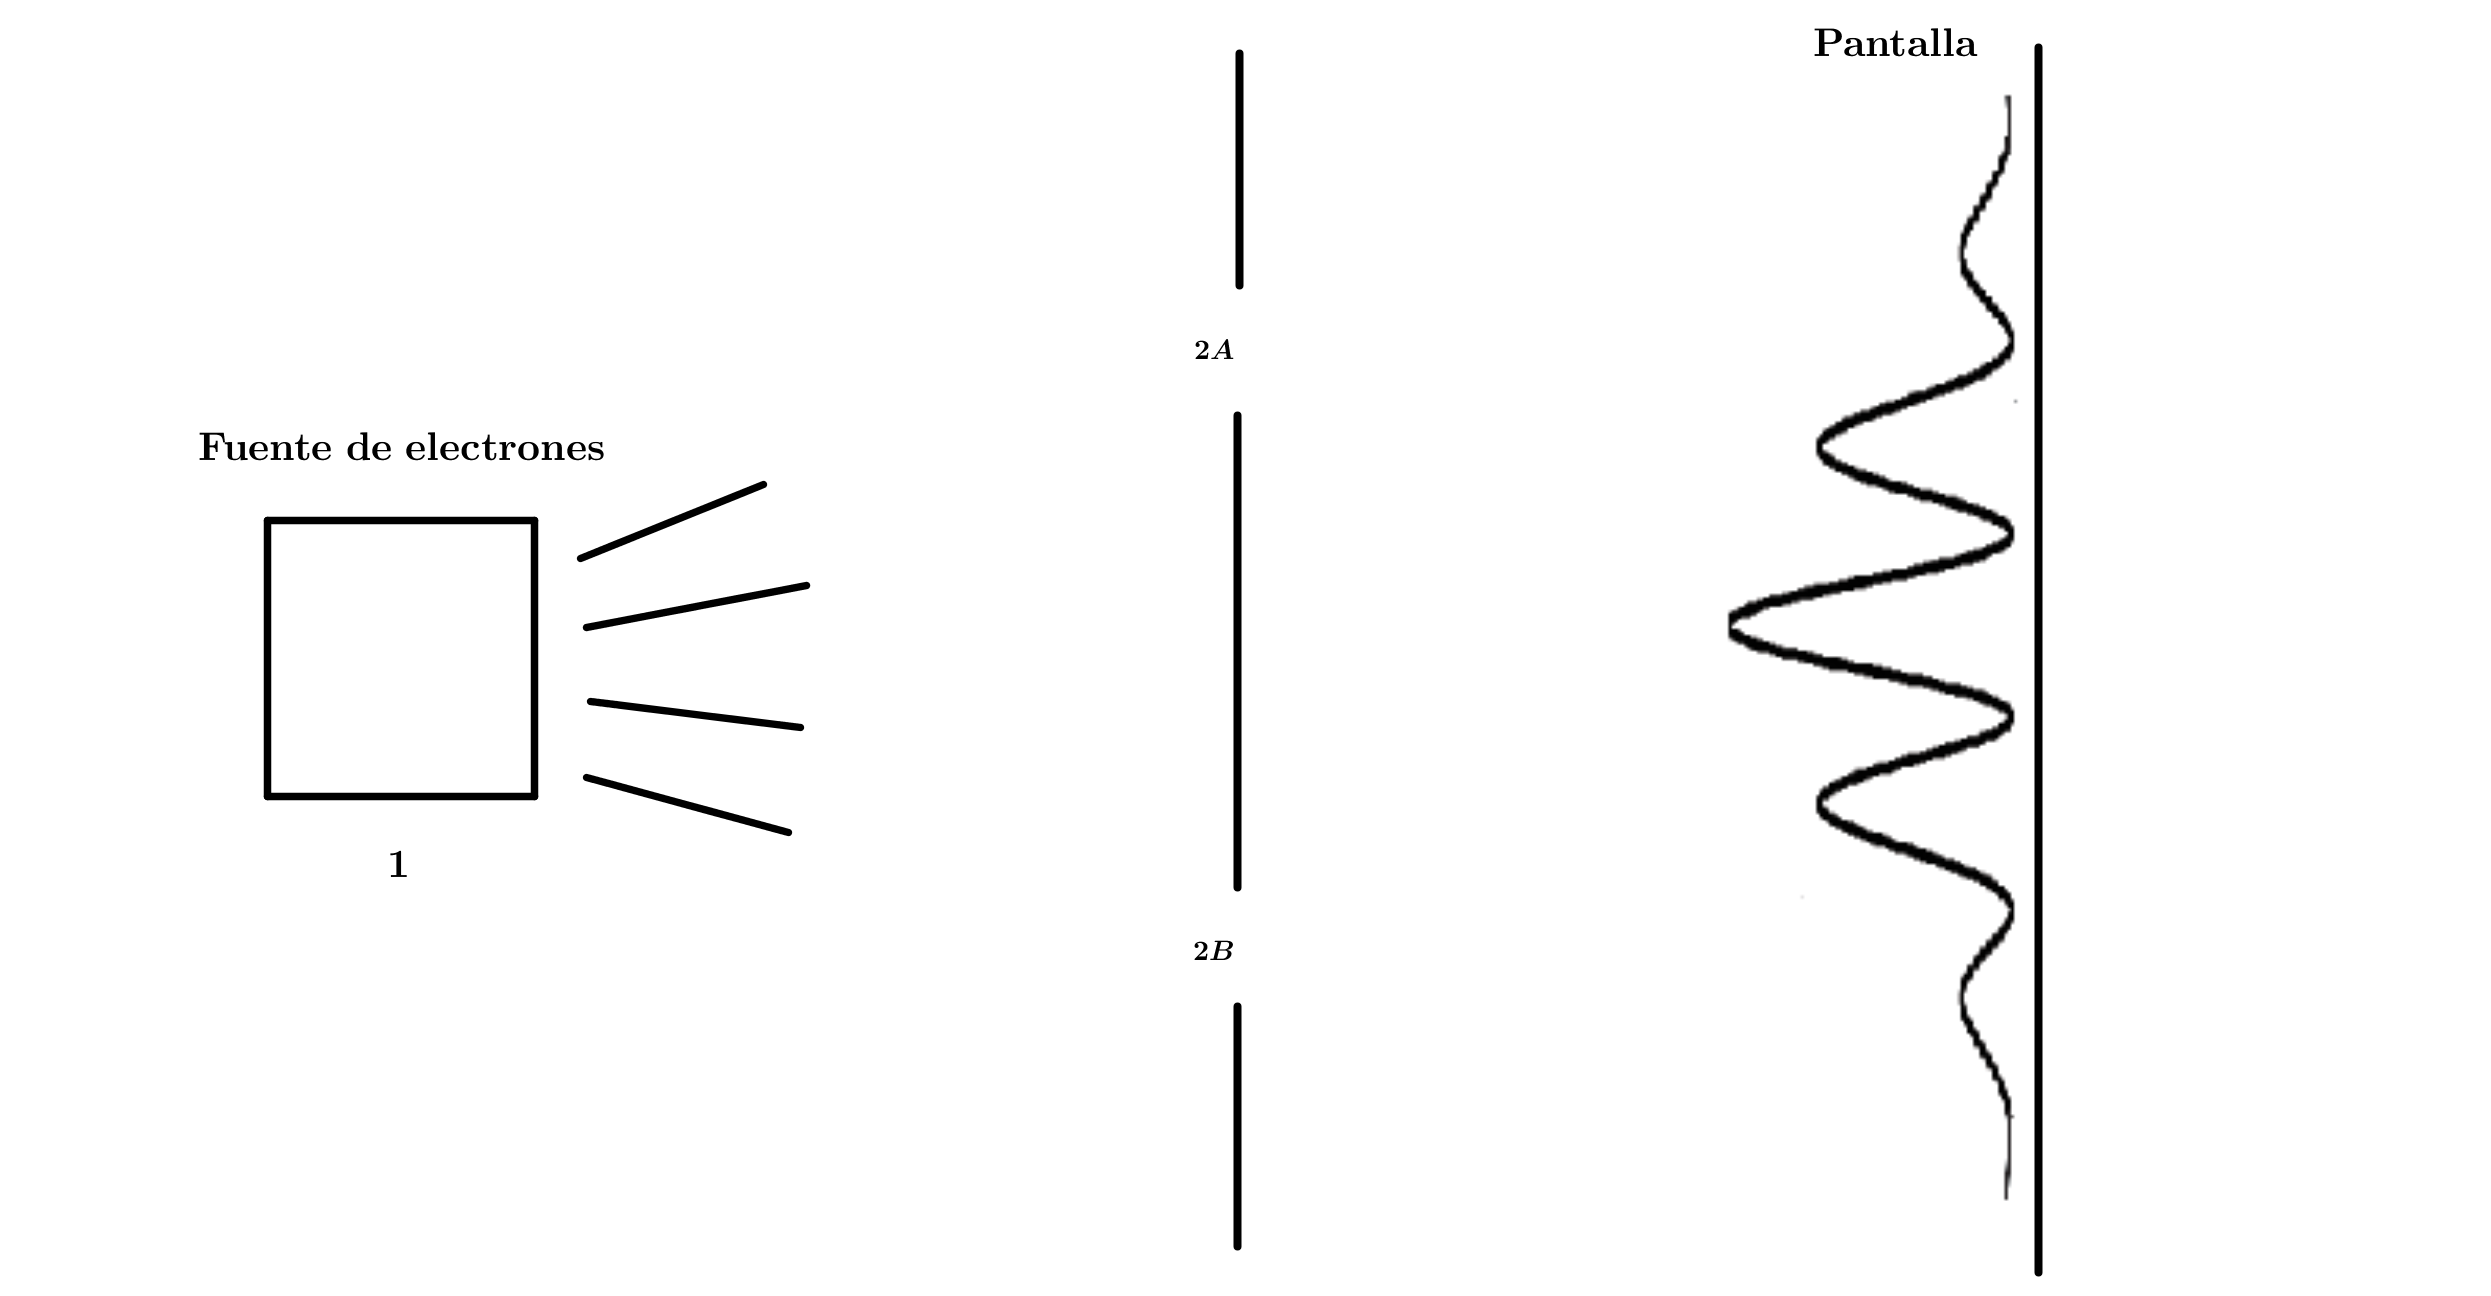
\includegraphics[width=9cm]{Imagenes/Fig1}
\caption[Esquema del experimento de la doble rendija]{Experimento de la doble rendija.}
\end{figure}
Si $K(2A,1)$ es la probabilidad de que un electrón pase por la rendija 2A, entonces podemos escribir:
\begin{equation}
K(3,1)=K(2A,1)K(3,2A)+K(2B,1)K(3,2B)
\end{equation}
Al tomar el módulo cuadrado de la expresión (2.5) se generarán los términos de interferencia necesarios para describir el patrón de difracción. No podemos decir que el electrón tomó un camino u el otro, de una manera más simple: este siguió todos los caminos posibles!

\section{La ecuación de Schrödinger.}
En el cuadro de Schrodinger la evolución de un sistema cuántico afecta al ket que representa al estado del sistema, la ecuación que rige la dinámica del mismo es la \textbf{Ecuación de Schrödinger}
\begin{equation}
i\hbar\frac{\partial}{\partial t}|\psi\rangle_S=\hat{H}|\psi\rangle_S
\end{equation}
Sabemos que $\psi(q,t)=\langle q|\psi \rangle_S$ donde $|q\rangle$ son autoestados de la posición, la relacion entre el cuadro de Heisenberg y el de Schrödinger es $|\psi\rangle_H=e^{iHt/\hbar}|\psi\rangle_S$. Si definimos $|qt\rangle \equiv e^{iHt/\hbar}|q\rangle$, entonces $\psi (q,t)=\langle qt|\psi\rangle_H$.

Vamos a mostrar que $K(q_f,t_f;q_i,t_i)=\left\langle q_ft_f|q_it_i \right\rangle$, la relación de completez nos permite escribir:
\begin{eqnarray}
\nonumber \langle q_ft_f|\psi\rangle &=& \int\langle q_ft_f|q_it_i\rangle\langle q_it_i|\psi\rangle dq_i\\
&=& \int \langle q_ft_f|q_it_i\rangle \psi(q_i,t_i)dq_i
\end{eqnarray}
Y comparando (2.7) y (2.2), vemos que:
\begin{equation}
K(q_f,t_f;q_i,t_i)=\langle q_ft_f|q_it_i\rangle
\end{equation}
Así, el propagador es proporcional a la amplitud de probabilidad de transición entre el estado inicial $|q_it_i\rangle$ y final $|q_ft_f\rangle$. La idea ahora es expresar el propagador como una integral de trayectoria. Partamos el intervalo temporal $(t_i,t_f)$ en $n+1$ piezas de igual duración $\tau$, así:
\begin{equation}
\langle q_ft_f|q_it_i\rangle \int dq_1dq_2...dq_n\langle q_ft_f|q_nt_n\rangle \langle q_nt_n|q_{n-1}t_{n-1}\rangle...\langle q_1t_1|q_it_i\rangle
\end{equation}
Calculemos uno de estos elementos:
\begin{eqnarray}
\nonumber \langle q_{j+1}t_{j+1}|q_jt_j\rangle &=&\langle q_{j+1}|e^{-iHt_{j+1}/\hbar}e^{iHt_j/\hbar}|q_j=\langle q_{j+1}|e^{-i\tau H/\hbar}|q_j\rangle \hspace{0.4cm}\text{A primer orden,}\\
\nonumber &=&\langle q_{j+1}|1-i\tau H/\hbar|q_j\rangle=\delta(q_{j+1}-q_j)-i\tau\hbar\langle q_{j+1}|H|q_j\rangle\\
&=& \frac{1}{2\pi\hbar}\int dp\ \text{Exp}[\frac{ip}{\hbar}(q_{j+1}-q_j)]-\frac{i\tau}{\hbar}\langle q_{j+1}|H|q_j\rangle 
\end{eqnarray}	
Si asumimos que el Hamiltoniano es una función de $p$ y $q$de la forma: $H=\frac{p^2}{2m}+V(q)$, entonces:
\begin{eqnarray}
\nonumber \langle q_{j+1}|\frac{p^2}{2m}|q_j \rangle &=& \int dpdp\prime \langle q_{j+1}|p\prime\rangle\langle p\prime|\frac{p^2}{2m}|p\rangle \langle p|q_j \rangle\\
\nonumber &=&\int \frac{dpdp\prime}{2\pi\hbar}\ \text{Exp}[\frac{i}{\hbar}(p\prime q_{j+1}-pq_j)]\frac{p^2}{2m}\delta(p-p\prime)\\
&=& \int \frac{dp}{2\pi\hbar}\ \text{Exp}[\frac{i}{\hbar}p(q_{j+1}-q_j)]\frac{p^2}{2m}
\end{eqnarray}
De una manera similar:
\begin{eqnarray}
\nonumber \langle q_{j+1}|V(q)|q_j \rangle &=& V(\frac{q_{j+1}+q_j}{2})\langle q_{j+1}|q_j\rangle\\
\nonumber &=& V(\frac{q_{j+1}+q_j}{2})\delta(q_{j+1}-q_j)\\
\langle q_{j+1}|V(q)|q_j \rangle &=& V(\frac{q_{j+1}+q_j}{2})\int \frac{dp}{2\pi\hbar}\ \text{Exp}[\frac{i}{\hbar}p(q_{j+1}-q_j)]
\end{eqnarray}
Por tanto $\langle q_{j+1}|H|q_j\rangle=\int \frac{dp}{h}\ \text{Exp}[\frac{i}{h}p(q_{j+1}-q_j)]H(p,q)$ y:
\begin{equation}
\langle q_{j+1}t_{j+1}|q_jt_j\rangle=\frac{1}{h}\int dp_j\ \text{Exp}[\frac{i}{\hbar}[p_j(q_{j+1}-q_j)-\tau H(p_j,q_j)]]
\end{equation}
Finalmente:
\begin{equation}
\langle q_{f}t_{f}|q_it_i\rangle=\lim_{N \to \infty}\int\prod_{j=1}^{N}dq_j\prod_{j=0}^{N}\frac{dp_j}{h}\ \text{Exp}\left\{ \frac{i}{\hbar}\sum_{j=0}^{N}[p_{j}(q_{j+1}-q_{j})-\tau H(p_{j},q_{j})]\right\}
\end{equation}
En el continuo:
\begin{equation}
\langle q_{f}t_{f}|q_it_i\rangle=\int\frac{\mathcal{D}q\mathcal{D}p}{h}\text{Exp\ensuremath{\left\{ \frac{i}{\hbar}\int_{t_{i}}^{t_{f}}(p\dot{q}-H(p,q))dt\right\} }}
\end{equation}
En el continuo $q$ se vuelve una función de $t$ y la integral anterior, es una integral funcional. La expresión (2.15) es la integral de trayectoria para la amplitud de transición entre $(q_i,t_i)$ y $(q_f,t_f)$. Esta integral se hace sobre todas las posibles trayectorias en el espacio de fase y $q(t), p(t)$ son funciones y no operadores, sin embargo es natural preguntarse por la convergencia de (2.15), esto es algo no trivial, sin embargo, de ahora en adelante asumiremos que esta integral existe y converge. 	
\\
Si el Hamiltoniano es tal que $H=\frac{p^2}{2m}+V(q)$
\begin{equation}
\langle q_{f}t_{f}|q_it_i\rangle=\lim_{N \to \infty}\int\prod_{j=1}^{N}dq_j\prod_{j=0}^{N}\frac{dp_j}{h}\ \text{Exp}\left\{ \frac{i}{\hbar}\sum_{j=0}^{N}[p_{j}(q_{j+1}-q_{j})-\tau \frac{p_j^2}{2m}-V(q)\tau]\right\}
\end{equation}
Y sabiendo que: $\int_{-\infty}^{\infty}\text{Exp}[-ax^{2}+bx+c]dx=\text{Exp}[\frac{b^{2}}{4a}+c](\frac{\pi}{a})^{\frac{1}{2}}$, entonces:
\begin{equation}
\langle q_{f}t_{f}|q_it_i\rangle=\lim_{N\to\infty}[\frac{1}{h}(\frac{\text{\ensuremath{\pi\hbar}2m}}{i\tau})^{\frac{1}{2}}]^{N+1}\int\prod_{1}^{N}dq_{j}\text{Exp}\left\{ \frac{i}{\hbar}\sum_{0}^{N}\left((\frac{q_{j+1}-q_{j}}{\tau})^{2}\frac{m}{2}-V\right)\tau\right\} 
\end{equation}
En el continuo:
\begin{equation}
\langle q_{f}t_{f}|q_it_i\rangle=\mathcal{N}\int\mathcal{D}q\text{Exp\ensuremath{\left\{ \frac{i}{\hbar}\int_{t_{i}}^{t_{f}}\mathcal{L}(q,\dot{q})dt\right\} }}
\end{equation}
Donde $\mathcal{L}(q,\dot{q})$ es el lagrangiano clásico, sin embargo esto solo pasa si asumimos una forma específica del Hamiltoniano, cuando esto no es asi se tiene una acción efectiva. En teorñia de campos por ejemplo esta descomposición solo se puede hacer en el caso de campos Abelianos.
\newpage
 
 

\subsection{Teoría de perturbaciones.}

Vamos a ilustrar cómo usar el método de integrales de trayectoria en procesos de dispersión, este tipo de procesos involucran la interacción de una partícula con un potencial $V(x)$. Debido a que no siempre podemos calcular analíticamente la integral (2.18) entonces es necesario acudir a la teoría de perturbaciones, esta es aplicable en el regimen en que la energía de interacción $E_I<\hbar$. En este caso podemos escribir:
\begin{equation}
\text{Exp}\left[\frac{-i}{\hbar}\int_{t_{i}}^{t_{f}}V(x,t)dt\right]=1-\frac{i}{\hbar}\int_{t_{i}}^{t_{f}}V(x,t)dt+\left(\frac{i}{\hbar}\right)^{2}\frac{1}{2!}\left[\int_{t_{i}}^{t_{f}}V(x,t)dt\right]^{2}+...
\end{equation}
Cuando reemplazamos esto en la expresión (2.18) obtenemos:
\begin{equation}
K=K_0+K_1+K_2+...\ \text{donde}\ K_0=\mathcal{N}\int \mathcal{D}x \text{Exp}\left[ \frac{i}{\hbar}\int \frac{1}{2}m\dot{x}^2dt\right] 
\end{equation}
Para calcular $K_0$, escribamos la forma discretizada de (2.20)
\begin{eqnarray}
\nonumber K_0&=&\lim_{n\to\infty}\left(\frac{m}{i\hbar\tau}\right)^{\left(\frac{n+1}{2}\right)}\int_{-\infty}^{\text{\ensuremath{\infty}}}\prod_{j=1}^{n}dx_{j}\text{Exp}\left[\frac{im}{2\hbar\tau}\sum_{j=0}^{n}\left(x_{j+1}-x_{j}\right)^{2}\right]\\
\nonumber &=& \lim_{n\to\infty}\left(\frac{m}{i\hbar\tau}\right)^{\left(\frac{n+1}{2}\right)}\frac{1}{\left(n+1\right)^{\frac{1}{2}}}\left(\frac{i\hbar\tau}{m}\right)^{\frac{n}{2}}\text{Exp}\left[\frac{im}{2\hbar(n+1)\tau}\left(x_{f}-x_{i}\right)^{2}\right]\\
K_0(x_ft_f,x_it_i)&=& \Theta(t_{f}-t_{i})\left(\frac{m}{i\hbar(t_{f}-t_{i})}\right)^{1/2}\text{Exp}\left[\frac{im}{2\hbar(t_{f}-t_{i})}\left(x_{f}-x_{i}\right)^{2}\right] 
\end{eqnarray}
Calculemos ahora $K_1$:
\begin{equation}
K_1=\lim_{n\to\infty}\frac{-i}{\hbar}N^{(n+1)/2}\sum_{i=1}^{n}\int\text{Exp}\left[\frac{im}{2\hbar\tau}\sum_{j=0}^{n}(x_{j+1}-x_{j})^{2}\right]V(x_{i},t_{i})dx_{1}...dx_{n}
\end{equation}
Ahora como solo $V(x)$ depende de $x_i$, separamos (2.22) como:
\begin{eqnarray}
\nonumber K_1&=&\lim_{n\to\infty}\frac{-i}{\hbar}\sum_{i=1}^{n}\left\{ \int N^{(n-i+1)/2}\text{Exp}\left[\frac{im}{2\hbar\tau}\sum_{j=i}^{n}(x_{j+1}-x_{j})^{2}\right]dx_{i}...dx_{n}\right\}\\
& &\times  \left\{ \int N^{i/2}\text{Exp}\left[\frac{im}{2\hbar\tau}\sum_{j=0}^{i-1}(x_{j+1}-x_{j})^{2}\right]dx_{1}...dx_{i-1}\right\} V(x_{i},t_{i})
\end{eqnarray}
Los dos términos en corchetes en (2.23) son $K_0(xt,x_ft_f)$ y $K_0(x_it_i,xt)$, así:
\begin{equation}
K_1(x_ft_f,x_it_i)= -\frac{i}{\hbar}\int_{t_{i}}^{t_{f}}dt\int_{-\infty}^{\infty}K_{0}(x_{f}t_{f}.xt)V(x,t)K_{0}(xt,x_{i}t_{i})dx
\end{equation}
Como $K_0(x_ft_f,xt)=0$ si $t>t_f$ y $K_0(xt,x_it_i)=0$ si $t<t_i$, entonces podemos escribir:
\begin{equation}
K_1(x_ft_f,x_it_i)=-\frac{i}{\hbar}\int_{-\infty}^{\infty}dt\int_{-\infty}^{\infty}K_{0}(x_{f}t_{f}.xt)V(x,t)K_{0}(xt,x_{i}t_{i})dx 
\end{equation}
De la misma manera se puede probar que:
\begin{equation}
K_2(x_ft_f,x_it_i)=\left(\frac{-i}{\hbar}\right)^2\int_{-\infty}^{\infty}dt_{1}dt_{2}dx_{1}dx_{2}K_{0}(x_{f}t_{f}.x_{2}t_{2})V_2K_{0}(x_{2}t_{2},x_{1}t_{1})V_1K_{0}(x_{1}t_{1},x_{i}t_{i})
\end{equation}
Esta es una solución en series para $K$ y recibe el nombre de Serie de Born, en la expresión general para $K_n$ no se tiene el factor $n!$ ya que hay ese mismo numero de formas para ordenar los $n$ potenciales $V(x)$ que entran en el propagador.
\\
\\
Por último mostraremos que \textbf{el propagador es la función de Green de la ecuación de Schrödinger.} Para esto sustituyamos la expresión para la serie de Born en la ecuación (2.2):
\begin{eqnarray}
\nonumber \psi(\vec{x}_f,t_f)&=&\int K_{0}(\vec{x_{f}}t_{f},\vec{x_{i}}t_{i})\psi(\vec{x_{i}},t_{i})d\vec{x_{i}}\\
& & \frac{-i}{\hbar}\int K_{0}(\vec{x_{f}}t_{f},\vec{x}t)V(\vec{x},t)K_{0}(\vec{x}t,\vec{x_{i}}t_{i})\psi(\vec{x_{i}},t_{i})d\vec{x}dtd\vec{x_{i}}+O(\hbar^{2})
\end{eqnarray}
Hemos cambiado a tres dimensiones espaciales y los otros términos en la serie hacen converger el último $K_0$ a $K$, por tanto:
\begin{equation}
\psi(\vec{x}_f,t_f)=\int K_{0}(\vec{x_{f}}t_{f},\vec{x_{i}}t_{i})\psi(\vec{x_{i}},t_{i})d\vec{x_{i}}-\frac{i}{\hbar}\int K_{0}(\vec{x_{f}}t_{f},\vec{x}t)V(\vec{x},t)\psi(\vec{x},t)d\vec{x}dt
\end{equation}
Cuando $t_i \to -\infty$,no hay presencia de potencial por tanto $\psi$ se vuelve una onda plana. Así:
\begin{equation}
\psi(\vec{x}_f,t_f)=\phi(\vec{x}_ft_f)-\frac{i}{\hbar}\int K_{0}(\vec{x_{f}}t_{f},\vec{x}t)V(\vec{x},t)\psi(\vec{x},t)d\vec{x}dt
\end{equation}
Aplicando el operador $\hat{H}=\frac{\hbar^2}{2m}\nabla_{\vec{x}_ft_f}+i\hbar\frac{\partial}{\partial t_f}$ en la ecuación (2.29) y usando $\hat{H}\psi(x,t)=V(x,t)\psi(x,t)$:
\begin{eqnarray}
\nonumber \hat{H}(\psi(\vec{x}_f,t_f))&=&\hat{H}(\phi(\vec{x}_ft_f))-\frac{i}{\hbar}\int\hat{H} (K_{0}(\vec{x_{f}}t_{f},\vec{x}t))V(\vec{x},t)\psi(\vec{x},t)d\vec{x}dt\\
\nonumber V(\vec{x}_f,t_t)\psi(\vec{x}_f,t_f)&=&0-\frac{i}{\hbar}\int\hat{H} (K_{0}(\vec{x_{f}}t_{f},\vec{x}t))V(\vec{x},t)\psi(\vec{x},t)d\vec{x}dt
\end{eqnarray}
Por tanto:
\begin{equation}
\left(\frac{\hbar^2}{2m}\nabla_{\vec{x}_ft_f}+i\hbar\frac{\partial}{\partial t_f}\right)K_{0}(\vec{x_{f}}t_{f},\vec{x}t)=i\hbar\delta(\vec{x}-\vec{x}_f)\delta(t-t_f)
\end{equation}
Esto último era lo que queríamos probar.








\subsection{Matriz $\mathcal{S}$.}
En un experimento de dispersión es razonable suponer que las partículas al principio y al final del proceso son partículas libres, estas ondas planas están distribuidas en todo el espacio. Sin embargo esto último lleva a una contradicción ya que la presencia del centro dispersor no permite que en sus cercanias la solución sea una onda plana. Para resolver este inconveniente se puede proponer lo que se llama una fuente dinámica, que se "prenda y apague" lentamente tal que las partículas en los estados (final/incial) puedan ser libres y por tanto la aproximación de ondas planas sea válida en este regimen.\\
\\
Para empezar definamos $\psi_{in}(\vec{x}_i,t_i)$, $\psi_{out}(\vec{x}_f,t_f)$ como ondas planas para $t\to -\infty$,  $t\to \infty$ respectivamente, la amplitud de dispersión se define como:
\begin{equation}
\mathcal{S}=\int\psi_{out}^{*}(\vec{x}_{f}t_{f})\psi^{(+)}(\vec{x}_{f}t_{f})d\vec{x}_{f}
\end{equation}
En (2.31) el superíndice $(+)$ denota que $\psi^{(+)}(\vec{x}t)$ era una onda libre en $t\to -\infty$, usando la serie de Born obtenemos:
\begin{eqnarray}
\nonumber \mathcal{S}&=&\int\psi_{out}^{*}(\vec{x}_{f}t_{f})\psi^{(+)}(\vec{x}_{f}t_{f})d\vec{x}_{f}=\int\psi_{out}^{*}(\vec{x}_{f}t_{f})K_{0}(\vec{x}_{f}t_{f},\vec{x}_{i}t_{i})\psi_{in}(\vec{x}_{i}t_{i})d\vec{x}_{f}d\vec{x_{i}}\\
\nonumber &&-\frac{i}{\hbar}\int\psi_{out}^{*}(\vec{x}_{f}t_{f})K_{0}(\vec{x}_{f}t_{f},\vec{x}t)V(\vec{x}t)K_{0}(\vec{x}t,\vec{x}_{i}t_{i})\psi_{in}(\vec{x}_{i}t_{i})d\vec{x}_{f}d\vec{x_{i}}d\vec{x}dt\\
\nonumber &=&\int \psi_{out}^{*}(\vec{x}_{f}t_{f})\phi(\vec{x}_{f}t_{f})d\vec{x}_f\\
&&-\frac{i}{\hbar}\int\psi_{out}^{*}(\vec{x}_{f}t_{f})K_{0}(\vec{x}_{f}t_{f},\vec{x}t)V(\vec{x}t)K_{0}(\vec{x}t,\vec{x}_{i}t_{i})\psi_{in}(\vec{x}_{i}t_{i})d\vec{x}_{f}d\vec{x_{i}}d\vec{x}dt   
\end{eqnarray}
Si los momentos iniciales y finales son $\vec{p}_i=\hbar\vec{k}_i$,$\vec{p}_f=\hbar\vec{k}_f$ respectivamente, entonces tenemos que:
\begin{eqnarray}
\psi_{in}(\vec{x}t)&=&\frac{1}{\sqrt{\tau}}\text{Exp}\left( \frac{i}{\hbar}(\vec{p}_i\cdot \vec{x}-E_it )\right)\\
\psi_{out}(\vec{x}t)&=&\frac{1}{\sqrt{\tau}}\text{Exp}\left( \frac{i}{\hbar}(\vec{p}_f\cdot \vec{x}-E_ft )\right)
\end{eqnarray}
Donde $E^2=\frac{p^2}{2m}$ y $\tau$ es el volumen de integración, el cual es arbitrario. Si sustituimos las expresiones (2.33) y (2.34) en (2.32) obtenemos:
\begin{equation}
\mathcal{S}_{fi}=\delta(\vec{k}_f-\vec{k}_i)-\frac{i}{\hbar}\int\psi_{out}^{*}(\vec{x}_{f}t_{f})K_{0}(\vec{x}_{f}t_{f},\vec{x}t)V(\vec{x}t)K_{0}(\vec{x}t,\vec{x}_{i}t_{i})\psi_{in}(\vec{x}_{i}t_{i})d\vec{x}_{f}d\vec{x_{i}}d\vec{x}dt
\end{equation}
Lo cual nos permite ver la amplitud de dispersion $\mathcal{S}_{fi}$ como el elemento de una matriz, la \textbf{matriz $\mathcal{S}$ de dispersión}. En (2.35) el primer término solo es representativo cuando no hay interacción y $\vec{k}_i=\vec{k}_f$. Las interacciones están representadas en el segundo término.\\
\\
Es posible representar este segundo término mediante una serie de diagramas a los cuales se les asocian ciertas reglas, estos diagramas reciben el nombre de \textbf{Diagramas de Feynmann}. Si nombramos:
\begin{equation}
\mathcal{A}=-\frac{i}{\hbar}\int\psi_{out}^{*}(\vec{x}_{f}t_{f})K_{0}(\vec{x}_{f}t_{f},\vec{x}t)V(\vec{x}t)K_{0}(\vec{x}t,\vec{x}_{i}t_{i})\psi_{in}(\vec{x}_{i}t_{i})d\vec{x}_{f}d\vec{x_{i}}d\vec{x}dt
\end{equation}

\begin{SCfigure}[1.3][h]
\caption[Diagrama de Feynmann primera cuantización]{Representación de $\mathcal{A}$}
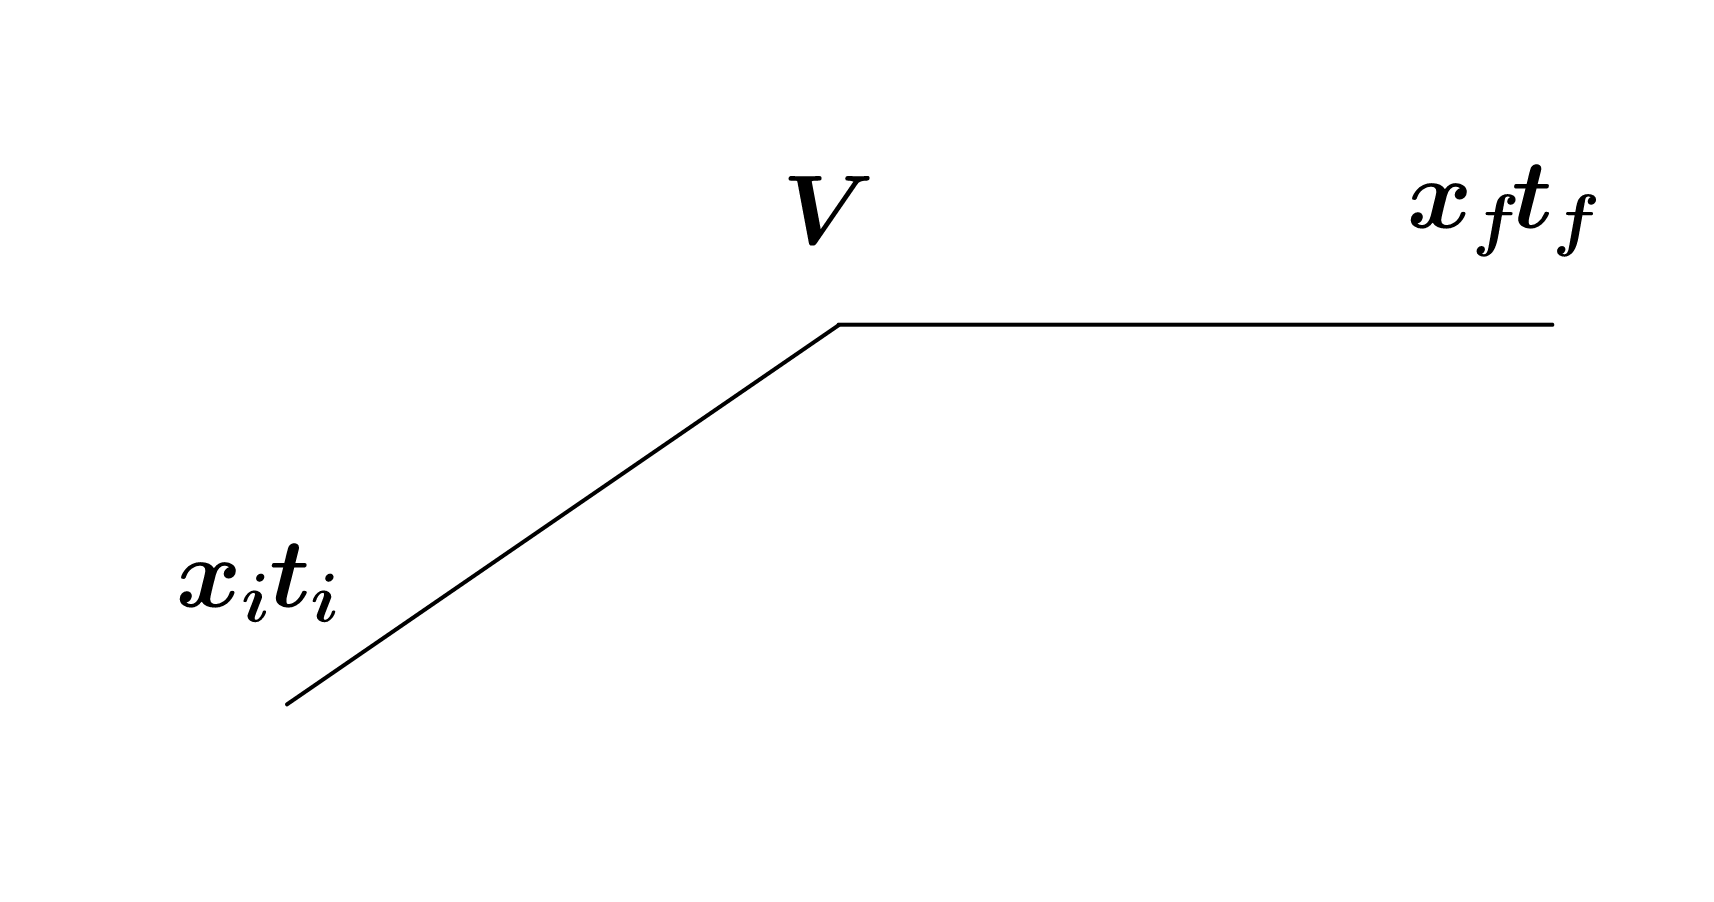
\includegraphics[width=4cm]{Imagenes/Fig2}
\end{SCfigure}
Este diagrama lo podemos descomponer usando la siguiente convención:
\begin{SCfigure}[1.3][h]
\caption[Diagrama de Feynmann primera cuantización]{Representación de $K_0(x_2t_2,x_1t_1)$}
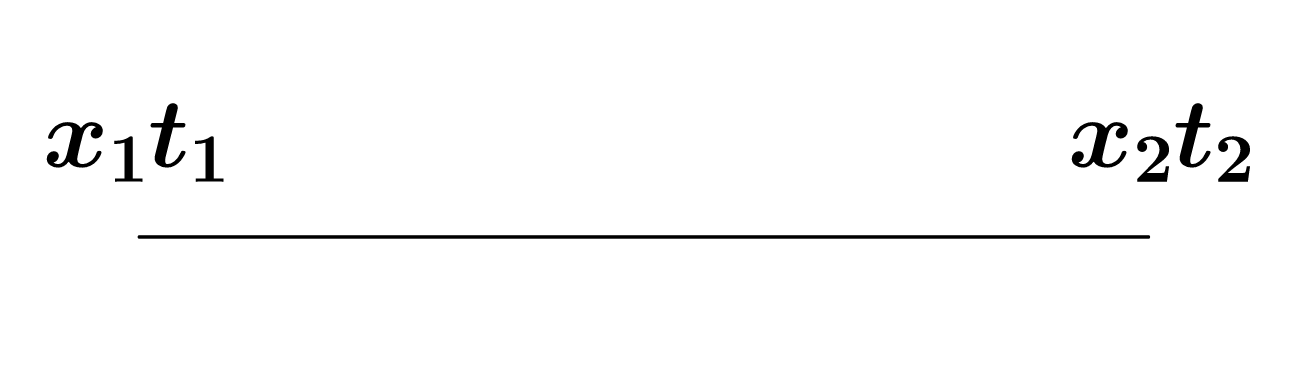
\includegraphics[width=4cm]{Imagenes/Fig3}
\end{SCfigure}
\begin{SCfigure}[1.3][h]
\caption[Diagrama de Feynmann primera cuantización]{Representación de $\int -\frac{i}{\hbar}V(xt)dxdt$}
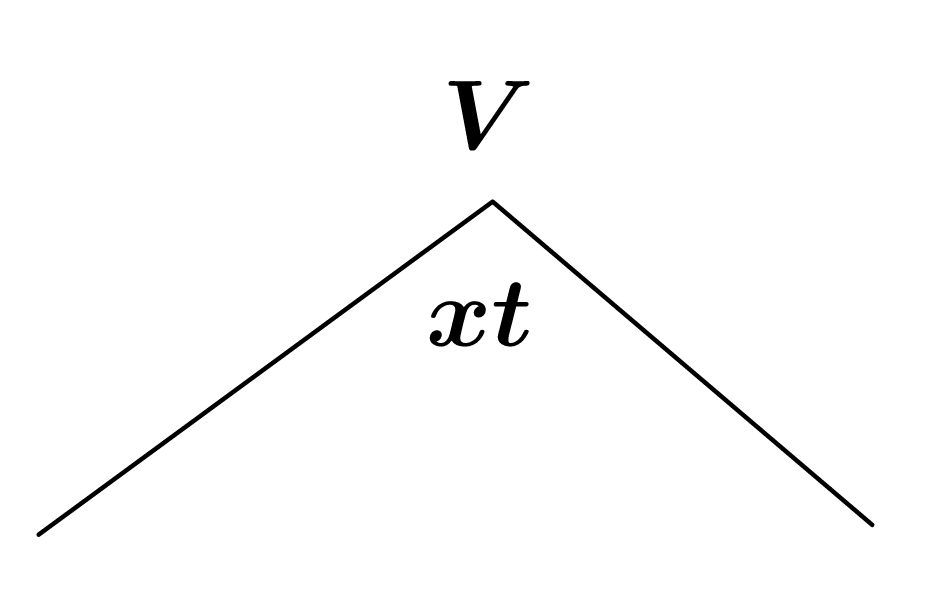
\includegraphics[width=4cm]{Imagenes/Fig4}
\end{SCfigure}
\\
Por ejemplo el diagrama correspondiente a término de segundo orden:
\begin{eqnarray}
\nonumber \mathcal{A}^{(2)}&=&\left(-\frac{i}{\hbar}\right)^2\int d\vec{x}_{f}d\vec{x_{i}}d\vec{x\prime}dt\prime d\vec{x}dtK_{0}(\vec{x}t,\vec{x}_it_i)V(\vec{x}t)K_{0}(\vec{x}\prime t\prime,\vec{x}t)\\
&&\times V(\vec{x}\prime t\prime)K_{0}(\vec{x}_{f}t_{f},\vec{x}\prime t\prime)\psi_{out}^{*}(\vec{x}_{f}t_{f})\psi_{in}(\vec{x}_{i}t_{i})
\end{eqnarray}
Es el siguiente:
\begin{SCfigure}[1.3][h]
\caption[Diagrama de Feynmann primera cuantización]{Representación de $\mathcal{A}^{(2)}$}
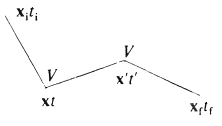
\includegraphics[width=4cm]{Imagenes/Fig5}
\end{SCfigure}
En algunos casos es útil conocer una expresión para el propagador  $K_0$en el espacio de momentos, definimos $\mathcal{K}_0(\vec{p}_1t_1,\vec{p}_2t_2)$ como la amplitud de que una partícula con momento $\vec{p}_2$ en un instante $t_2$, sea observada un instante de tiempo después en $t_1$ con momento $\vec{p}_1$. Así:
\begin{eqnarray}
\nonumber \mathcal{K}_0(\vec{p}_1t_1,\vec{p}_0t_0)&=&\int \text{Exp}\left(\frac{-i}{\hbar}(\vec{p}_1\cdot\vec{x}_1)\right) K_0(\vec{x}_1t_1,\vec{x}_0t_0)\text{Exp}\left(\frac{-i}{\hbar}(\vec{p}_0\cdot\vec{x}_0)\right)d\vec{x}_0d\vec{x}_1\\
&&\nonumber \Theta(t_{1}-t_{0})\left(\frac{m}{i\hbar(t_{1}-t_{0})}\right)^{1/2}\int\text{Exp}\left[\frac{i}{\hbar}(\vec{p}_{0}\cdot\vec{x}_{0}-\vec{p}_{1}\cdot\vec{x}_{1})\right]\\
&& \times \text{Exp}\left[\frac{im(\vec{x}_{0}-\vec{x}_{1})^{2}}{2\hbar(t_{1}-t_{0})}\right]d\vec{x}_{0}d\vec{x}_{1}
\end{eqnarray}
Ahora si introducimos las siguientes variables:
\begin{equation}
\vec{x}=\vec{x}_0-\vec{x}_1;\hspace{0.3cm}\vec{X}=\vec{x}_0+\vec{x}_1;\hspace{0.3cm}\vec{p}=\vec{p}_0-\vec{p}_1;\hspace{0.3cm}\vec{P}=\vec{p}_0+\vec{p}_1
\end{equation}
Teniendo en cuenta que el Jacobiano de esta transformación es $J=\left(\frac{1}{2}\right)^3=\frac{1}{8}$ y con $\alpha=\frac{m}{2\hbar (t_1-t_0)}$  podemos escribir:
\begin{equation}
\mathcal{K}_0(\vec{p}_1t_1,\vec{p}_0t_0)=\Theta(t_{1}-t_{0})\left(\frac{\alpha}{i\pi}\right)^{3/2}\frac{1}{8}\int\text{Exp}\left[\frac{i\vec{p}\cdot\vec{X}}{2\hbar}\right]d\vec{X}\int\text{Exp}\left[\frac{i\vec{P}\cdot\vec{x}}{2\hbar)}\right]e^{i\alpha x^{2}}d\vec{x}
\end{equation}
La primera integral es $I_1=8(2\pi\hbar)^3\delta(\vec{p}_0-\vec{p}_1)$, la segunda la podemos calcular con la identidad $ \int e^{-ax^2+bx+c}=e^{\frac{b^2}{4a}+c}\left(\frac{\pi}{a}\right)^(1/2)$, por tanto $I_2=\left(\frac{i\pi}{\alpha}\right)^{3/2}\text{Exp}\left[\frac{-i\vec{P}^{2}}{8\hbar^{3}4i\alpha}\right]$, por tanto:
\begin{equation}
\mathcal{K}_0(\vec{p}_1t_1,\vec{p}_0t_0)=(2\pi\hbar)^3\Theta(t_1-t_0)\delta(\vec{p}_1-\vec{p}_0)\text{Exp}\left[\frac{-i\vec{P}^{2}(t_{1}-t_{0})}{8m\hbar}\right]
\end{equation}
Si también realizamos la transformada de Fourier en el tiempo, obtenemos:
\begin{equation}
\mathcal{K}_0(\vec{p}_1E_1,\vec{p}_0E_0)=(2\pi\hbar)^4\delta(\vec{p}_0-\vec{p}_1)\delta(E_1-E_0)\frac{i\hbar}{E-\frac{p_{1}^{2}}{2m}+i\epsilon}
\end{equation}
De aquí las reglas de Feynmann en el espacio de momentos son:
\begin{SCfigure}[1.3][h]
\caption[Diagrama de Feynmann primera cuantización]{Representación de $\frac{1}{(2\pi\hbar)^4}\frac{i\hbar}{E-\frac{p_{1}^{2}}{2m}+i\epsilon}$}
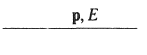
\includegraphics[width=4cm]{Imagenes/Fig6}
\end{SCfigure}
\begin{SCfigure}[1.3][h]
\caption[Diagrama de Feynmann primera cuantización]{Representación de $\frac{-i}{\hbar}(2\pi\hbar)^4v(\vec{q},W)$}
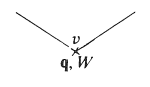
\includegraphics[width=4cm]{Imagenes/Fig7}
\end{SCfigure}

\subsection{Propiedades adicionales de las integrales de trayectoria.}
Ya hemos mostrado que la amplitud de transición entre un estado $(q_i,t_i)$ a $(q_f,t_f)$ está dada por:
\begin{equation}
\langle q_{f}t_{f}|q_it_i\rangle=\mathcal{N}\int\mathcal{D}q\text{Exp\ensuremath{\left\{ \frac{i}{\hbar}\int_{t_{i}}^{t_{f}}\mathcal{L}(q,\dot{q})dt\right\} }}
\end{equation}
En un experimento real, las partículas creadas en algún instante en el pasado son destruidas al ser detectadas, esto lo podemos interpretar de la siguiente manera: El estado de vacío en $t=-\infty$ evoluciona al mismo vacío en $t=\infty$. En este proceso una partícula es creada para ser posteriormente destruida, todo esto en presencia de una fuente generadora de estos procesos. Así es razonable poner nuestro interés en calcular transiciones vacío-vacío en presencia de una fuente.\\
\\
Podemos modificar el Lagrangiano de la de la siguiente manera: $\mathcal{L} \to \mathcal{L}+\hbar J(t)q(t)$. Si $|0,t\rangle^J $ es el estado fundamental en presencia de la fuente, entonces la amplitud de transición se define de la siguiente manera:
\begin{equation}
Z[J]\propto \langle 0,\infty|0,-\infty\rangle ^J
\end{equation}
La fuente $J(t)=0$ para $t>t\prime$ , $t\prime \prime < t$. Instroduzcamos entonces $T$ y $T\prime $ de tal manera que $T<t\prime\prime $ , $T\prime>t\prime $ por tanto la amplitud (2.44) es:
\begin{equation}
\langle 	Q\prime T\prime |QT\rangle=\mathcal{N}\int\mathcal{D}q\text{Exp\ensuremath{\left\{ \frac{i}{\hbar}\int_{T}^{T\prime}\mathcal{L}(q,\dot{q})dt\right\} }}
\end{equation}
Podemos escribir:
\begin{equation}
\langle Q\prime T\prime |QT \rangle^J=\int dq\prime dq\langle Q\prime T\prime | q\prime t\prime  \rangle\langle q\prime t\prime | qt \rangle\langle qt|QT \rangle
\end{equation}
Ahora si denotamos $|E_q\rangle$ como un autoestado del hamiltoniano podemos usar estos estados para expandir:
\begin{eqnarray}
\nonumber \langle Q\prime T\prime | q\prime t\prime  \rangle &=& \langle Q\prime|\text{Exp}\left[\frac{-i}{\hbar}HT\prime\right]\text{Exp}\left[\frac{i}{\hbar}Ht\prime\right]|q\prime\rangle\\
\nonumber &=& \sum_{mn}\phi^{*}(q\prime)\phi(Q\prime)\langle E_{Q\prime}|\text{Exp}\left[\frac{-i}{\hbar}HT\prime\right]\text{Exp}\left[\frac{i}{\hbar}Ht\prime\right]|E_{q\prime}\rangle\\
&=&\sum_{m}\phi^{*}(q\prime)\phi(Q\prime)Exp\left[\frac{i}{\hbar}E_{m}(t\prime-T\prime)\right]
\end{eqnarray}
De la misma manera:
\begin{equation}
\langle qt|	QT  \rangle=\sum_{m}\phi^{*}(Q)\phi(q)Exp\left[\frac{i}{\hbar}E_{m}(t-T)\right]
\end{equation}
Introduciendo (2.47) y (2.48) en (2.46):
\begin{eqnarray}
\nonumber \langle Q\prime T\prime|QT\rangle &=&\int dq\prime dq\sum_{m}\phi_{m}(Q\prime)\phi_{m}(q\prime,t)Exp\left[\frac{-i}{\hbar}E_{m}T\prime\right]\\
&&\times  \sum_{n}\phi_{n}^{*}(Q)\phi_{n}^{*}(q,t)Exp\left[\frac{i}{\hbar}E_{n}T\right]\langle q\prime t\prime|qt\rangle^{J}
\end{eqnarray}
Si hacemos una rotación de Wick de $T$ y $T\prime $ nos damos cuenta que el el término que menos sufre de supresión en la integral (2.49) es el asociado a $m=n=0$, por tanto:
\begin{equation}
\int dq\prime dq\phi_{0}^{*}(q\prime,t\prime)\langle q\prime t\prime|qt\rangle^{J}\phi_{0}(q,t)=\lim_{T\to-\text{\ensuremath{\infty}e}^{-i\delta},T\prime\to\text{\ensuremath{\infty}e}^{-i\delta}}\frac{\langle Q\prime T\prime|QT\rangle^{J}}{\phi_{0}^{*}(Q)\phi_{0}(Q\prime)\text{Exp}\left[\frac{-i}{\hbar}E_{0}(T\prime-T)\right]}
\end{equation}
El lado de (2.50) es simplemente el valor de expectación en el vacio de la amplitud de transcición, justo lo que buscabamos y el denominador de la parte derecha de la ecuación es simplemente una constante, así:
\begin{equation}
\langle 0,\infty| 0,-\infty \rangle ^J \propto \lim_{T\to-\text{\ensuremath{\infty}e}^{-i\delta},T\prime\to\text{\ensuremath{\infty}e}^{-i\delta}}\langle Q\prime T\prime|QT\rangle^{J}
\end{equation}
Otra forma equivalente de obtener este mismo resultado es: en vez de hacer una rotación de Wick, podemos agregar una pequeña cantidad imaginaria negativa al hamiltoniano $H+(-\frac{1}{2}i\epsilon q^2)$, lo cual es equivalente a restar esta misma cantidad a $\mathcal{L}$, de aquí que:
\begin{equation}
Z[J]=\int\mathcal{D}q\text{Exp\ensuremath{\left\{ \frac{i}{\hbar}\int_{-\infty}^{\infty}(\mathcal{L}(q,\dot{q})+\hbar Jq + \frac{1}{2}i\epsilon q^2)dt\right\} }}
\end{equation}
En general se cumple que:
\begin{equation}
 \langle q_{f}t_{f}|T[q(t_{1})...q(t_{n})]|q_{i}t_{i}\rangle=\mathcal{N}\int\mathcal{D}qq(t_{1})...q(t_{n})\text{Exp}\left[\frac{i}{\hbar}\int_{t_{i}}^{t_{f}}\mathcal{L}dt\right]
\end{equation}
Donde $T$ es el operador de ordenamiento temporal. Si derivamos funcionalmente la expresión para $Z[J]$ respecto a $J(t)$ obtenemos:
\begin{equation}
\frac{\delta Z[J]}{\delta J(t_{1}).}|_{J=0}=i\mathcal{N}\int\mathcal{D}qq(t_{1})\text{Exp}\left[\frac{i}{\hbar}\int_{t_{i}}^{t_{f}}\mathcal{L}dt\right]
\end{equation}	
Haciendo esto $n$ veces:
\begin{equation}
\frac{\delta^{n}Z[J]}{\delta J(t_{1})...\delta J(t_{n}).}|_{J=0}=i^{n}\mathcal{N}\int\mathcal{D}qq(t_{1})...q(t_{n})\text{Exp}\left[\frac{i}{\hbar}\int_{t_{i}}^{t_{f}}\mathcal{L}dt\right]
\end{equation}
De igualar las ecuaciones (2.53), (2.55) y al tener en cuenta agregar el factor $\frac{1}{2}i\epsilon q^2$ (el cual simplemente va a hacer converger los estados inicial y final en (2.53) a estados de vacío) obtenemos:
\begin{equation}
\frac{\delta^{n}Z[J]}{\delta J(t_{1})...\delta J(t_{n}).}|_{J=0}\propto i^{n}\langle0,\infty|T[q(t_{1})...q(t_{n})]|0,-\infty\rangle
\end{equation}
Estas últimas expresiones que hemos derivado van a ser importantes como punto de partida a la hora de tratar de cuantizar una teoría de campos vía el formalismo de integrales de trayectoria.
\newpage


\section{El experimento de la doble rendija.}
En esta sección aplicaremos lo aprendido en la $\mathsection$2.1 para resolver vía integrales de trayectoria el conocido problema de la difracción de electrones por una y dos rendijas. 

\subsection{El propagador de una partícula libre.}

Con este objetivo en mente primero necesitamos conocer el propagador de una partícula libre, sabemos que en un espacio plano de una dimensión la integral de trayectoria está dada por la expresión (2.17),podemos hacer facilmente una analogía para un espacio euclídeo d-dimensional. En este caso el propagador es:
\begin{eqnarray}
\nonumber K(x_{f}t_{f,},x_{i,}t_{i})&=&\lim_{n\to\infty}\frac{1}{(2\pi i\hbar\epsilon/m)^{d/2}}\prod_{k=1}^{n}\int\frac{d^{d}x_{k}}{(2\pi i\hbar\epsilon/m)^{d/2}}\\
&&\times \text{Exp}\left\{ \frac{i}{\hbar}\sum_{k=1}^{n}\epsilon\left[\frac{m(x_{k}-x_{k-1})^{2}}{2\epsilon^{2}}-V(x_{k})\right]\right\} 
\end{eqnarray}
donde $\epsilon=(t_i-t_f)/n$; para una partícula libre $V(x_k)=0$, entonces:
\begin{equation}
K(x_{f}t_{f,},x_{i,}t_{i})=\lim_{n\to\infty}\frac{1}{(2\pi i\hbar\epsilon/m)^{d/2}}\prod_{k=1}^{n}\int\frac{d^{d}x_{k}}{(2\pi i\hbar\epsilon/m)^{d/2}}\text{Exp}\left\{ \frac{i}{\hbar}\sum_{k=1}^{n}\left[\frac{m(x_{k}-x_{k-1})^{2}}{2\epsilon}\right]\right\}
\end{equation}
Para $d=1$, integremos los términos que tienen que ver con $x_1$:
\begin{eqnarray}
\nonumber &\frac{1}{(2\pi i\hbar\epsilon/m)^{1/2}}\prod_{k=1}^{n}\int\frac{dx_{1}}{(2\pi i\hbar\epsilon/m)^{1/2}}\text{Exp}\left\{ \frac{im(x_{1}-x_{0})^{2}}{2\hbar\epsilon}\right\} \text{Exp}\left\{ \frac{im(x_{2}-x_{1})^{2}}{2\hbar\epsilon}\right\}\\
\nonumber &=\frac{1}{(2\pi i\hbar\epsilon/m)}\int dx_{1}\text{Exp}\left\{ \frac{-m}{2i\epsilon\hbar}\left(2x_{1}^{2}-2x_{1}(x_{2}+x_{0})+x_{0}^{2}+x_{2}^{2}\right)\right\}\\
\nonumber &\text{Usando} \ \int e^{-ax^{2}+bx+c}dx=e^{^{\frac{b^{2}}{4a}+c}}\left(\frac{\pi}{a}\right)^{1/2}\\
\nonumber &=\frac{1}{\sqrt{2\pi i\hbar(2\epsilon)/m}}\text{Exp\ensuremath{\left\{ \frac{im(x_{2}-x_{0})^{2}}{2\hbar(2\epsilon)}\right\} }}
\end{eqnarray}
Ahora al seguir con la integral de $x_2$ queda:
\begin{eqnarray}
\nonumber & \frac{1}{(2\pi i\hbar\epsilon/m)\sqrt{2}}\int dx_{2}\text{Exp}\left\{ \frac{im}{2\hbar(2\epsilon)}\left(x_{2}-x_{o}\right)^{2}\right\} \text{Exp}\left\{ \frac{im}{2\hbar\epsilon}\left(x_{3}-x_{2}\right)^{2}\right\} \\
&=\frac{1}{\sqrt{2\pi i\hbar(3\epsilon)/m}}\text{Exp\ensuremath{\left\{ \frac{im(x_{3}-x_{0})^{2}}{2\hbar(3\epsilon)}\right\} }}
\end{eqnarray}
Así por inducción:
\begin{eqnarray}
\nonumber K(x_{f}t_{f},x_{i}t_{i})&=&\lim_{n\to\infty}\frac{1}{\sqrt{2\pi i\hbar(n\epsilon)/m}}\text{Exp\ensuremath{\left\{ \frac{im(x_{f}-x_{i})^{2}}{2\hbar(n\epsilon)}\right\} }}\\
&=& \frac{1}{\sqrt{2\pi i\hbar(t_{f}-t_{i})/m}}\text{Exp\ensuremath{\left\{ \frac{im(x_{f}-x_{i})^{2}}{2\hbar(t_{f}-t_{i})}\right\} }}
\end{eqnarray}
Por tanto en 3-D:
\begin{equation}
K^{3D}(x_{f}t_{f},x_{i}t_{i})\equiv K_{0}^{3D}=\left(\frac{m}{2\pi i\hbar(t_{f}-t_{i})}\right)^{3/2}\text{Exp\ensuremath{\left\{ \frac{im|\vec{x}_{f}-\vec{x}_{i}|^{2}}{2\hbar(t_{f}-t_{i})}\right\} }}
\end{equation}


\subsection{El problema de difracción e interferencia.}
Consideremos el siguiente experimento: una fuente de electrones en $(x,y,z)=(0,0,0)$ y dos rendijas en $Z=D$ con ancho $2a$ y centradas en $x=\pm b$, tal como se muestra en la figura 2.6. Adicionalmente consideramos que las barreras son lo suficientemente largas en $y$ como para poder despreciar los efectos de difracción inducidos en el caso de que estas fueran finitas.\\
\\
Así reducimos la dimensión del propagador en $y$:
\begin{eqnarray}
\nonumber K_{0}^{2D}(\vec{r}t,\vec{r}\prime t\prime)&=&\int_{-\infty}^{\infty}dyK_{0}^{3D}(\vec{r}t,\vec{r}\prime t\prime)\\
&=& \frac{m}{2\pi i\hbar(t-t\prime)}Exp\left\{ \frac{im|\vec{x}-\vec{x}\prime|^{2}}{2\hbar(t-t\prime)}\right\} 
\end{eqnarray}
Donde $|\vec{x}-\vec{x}\prime|^{2}$ se define como el módulo cuadrádo de la distancia en el plano $z-x$. Para modelar las rendijas vamos a usar las siguientes funciones escalón:
\[   
\chi_{[b-a,b+a]}(\omega) = 
     \begin{cases}
       0 &\omega>b+a,\omega<b-a\\
       1 &b-a<\omega<b+a \\
      
     \end{cases}
\]
La pregunta es. ¿cuál es la probabilidad de encontrar un electrón en ($z=L+D,x$)?, dado que haya salido de ($x=0,z=0$). Asumiendo que la fuente libera electrones individualmente podemos despreciar la interacción entre ellos.
\begin{figure}[h]
\centering
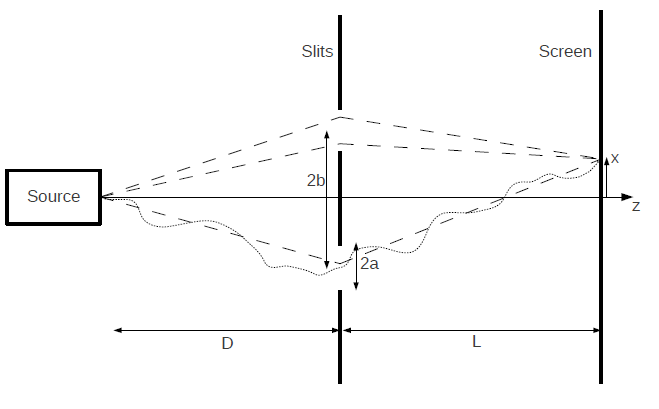
\includegraphics[width=10cm]{Imagenes/Fig8}
\caption[Esquema del experimento de la doble rendija en 2D]{Experimento de la doble rendija.}
\end{figure}
Como sabemos la probabilidad está dada por el módulo al cuadrado de la amplitud , la cual calcularemos usando el propagador. Como explicamos anteriormente hemos tomado $d=2$ en el propagador, sin embargo vamos a explicar por qué podemos reducir aún más la complejidad del problema: consideremos la difracción por una sola rendija y que el movimiento está dividido en dos regiones, uno empezando desde la fuente y llegando a las rendijas un tiempo $T$ despues de la emisión y otro de la rendija a la pantalla, este último de duración $\tau$.
\\
\\
Sin embargo no hay nada en las leyes de la mecánica cuántica que nos diga que podemos separar el movimiento en dos tramos, esto debido a que realmente no tenemos certeza de la posición de la partícula en un tiempo $T$. En pocas palabras no sabemos cuando el electrón ha cruzado la rendija.
\\
\\
No obstante podemos considerar esta imagen clásica para estudiar el problema, veamos por qué: el electrón tiene un momentum $p_z=\hbar k_z$, el cual esta relacionado con la velocidad clásica como $V_z=D/T=L/\tau$, aquí suponemos que $D$ es suficientemente grande comparado con las dimensiones en $x$ ($x,a,b\ll D,L$). Adicionalmente la longitud de onda $\lambda$ de la partícula es aproximadamente igual a la contribucion en $z$ (esto es como si tomaramos partículas que no se desvían demasiado de la trayectoria clásica). Si $\lambda \approx \lambda_z=2\pi\hbar/(mv_z)$ entonces $\lambda \ll D,L$. Esto quiere decir que el movimiento en $z$ es practicamente clásico. Note que cuánticamente es posible que el electrón pase a través de la rendija varias veces, sin embargo la probabilidad de este suceso ha de ser baja.

Teniendo en cuenta lo anterior:
\begin{eqnarray}
\nonumber K_{a,b}^{2D}((x,L+D),T+\tau;(0,0),0)&=&\int_{-\infty}^{\infty}d\omega\chi_{[b-a,b+a]}(\omega)K_{0}^{2D}((x,L+D),T+\tau;(\omega,D),T)\\
&&\nonumber \times K_{0}^{2D}((\omega,D),T;(0,0),0)\\
&=&\nonumber \frac{e^{\frac{imL^{2}}{2\hbar\tau}}}{\sqrt{2\pi i\hbar\tau/m}}\frac{e^{\frac{imD^{2}}{2\hbar T}}}{\sqrt{2\pi i\hbar T/m}}\int_{b-a}^{b+a}\frac{e^{\frac{im\omega^{2}}{2\hbar T}}}{\sqrt{2\pi i\hbar T/m}}\frac{e^{\frac{im(x-\omega)^{2}}{2\hbar\tau}}}{\sqrt{2\pi i\hbar\tau/m}}d\omega 	
\end{eqnarray}
Por tanto el propagador es el producto de dos propagadores independientes:
\begin{eqnarray}
K_z(L+D,T+\tau;0,0)&=&\frac{e^{\frac{imL^{2}}{2\hbar\tau}}}{\sqrt{2\pi i\hbar\tau/m}}\frac{e^{\frac{imD^{2}}{2\hbar T}}}{\sqrt{2\pi i\hbar T/m}}\\
K_x(x,T+\tau;0,0)&=&\int_{b-a}^{b+a}\frac{e^{\frac{im\omega^{2}}{2\hbar T}}}{\sqrt{2\pi i\hbar T/m}}\frac{e^{\frac{im(x-\omega)^{2}}{2\hbar\tau}}}{\sqrt{2\pi i\hbar\tau/m}}d\omega
\end{eqnarray}
Una forma de comprobar que las ecuaciones (2.63) y (2.64) son correctas es ver que si quitamos las rendijas ($a\to \infty$) e integramos en $D$ en el intervalo $(-\infty,\infty)$ recuperamos el propagador de una particula libre.\\
\\
En lo que sigue nos vamos a dar a la tarea de mostrar que podemos expresar la amplitud en términos de las conocidas integrales de Fressnel, sabemos que $P(x;a,b)=|A(x;a,b)|^2$ y de (2.64):
\begin{equation}
A_1(x;a,b)=\int_{b-a}^{b+a}\frac{e^{\frac{im\omega^{2}}{2\hbar T}}}{\sqrt{2\pi i\hbar T/m}}\frac{e^{\frac{im(x-\omega)^{2}}{2\hbar\tau}}}{\sqrt{2\pi i\hbar\tau/m}}d\omega
\end{equation} 
Organicemos de una manera diferente el exponencial de la ecuación (2.65):
\begin{eqnarray}
\nonumber \frac{m}{2\hbar\tau}(x-\omega)^{2}+\frac{m\omega^{2}}{2\hbar\tau}&=&\frac{m}{2\hbar}\left[\frac{1}{T}+\frac{1}{\tau}\right]\left[\omega^{2}-\frac{2x\omega}{\left(\frac{\tau}{T}+1\right)}+\left(\frac{x}{\frac{\tau}{T}+1}\right)^{2}-\left(\frac{x}{\frac{\tau}{T}+1}\right)^{2}\right]+\frac{mx^{2}}{2\text{\ensuremath{\hbar\tau}}}\\
&=&\nonumber \frac{m}{2\hbar}\left[\frac{1}{T}+\frac{1}{\tau}\right]\left[\omega-\frac{x}{1+\tau/T}\right]^{2}+\frac{mx^{2}}{2\text{\ensuremath{\hbar}}}\left[\frac{1}{\tau}-\frac{T}{(\tau+T)\tau}\right]\\
&=& \left[\frac{m}{2\hbar T}+\frac{m}{2\hbar\tau}\right]\left[\omega-\frac{x}{1+\tau/T}\right]^{2}+\frac{mx^{2}}{2\text{\ensuremath{\hbar}}(T+\tau)}
\end{eqnarray}
Por tanto reemplazando (2.66) en (2.65)
\begin{equation}
A_{1}(x;a,b)=\frac{e^{\frac{imx^{2}}{2\hbar(T+\tau)}}}{\sqrt{2\pi i\hbar(T+\tau)/m}}\int_{b-a}^{b+a}d\omega\sqrt{\frac{T+\tau}{2\pi\hbar T\tau/m}}\text{Exp}\left\{ \frac{i(T+\tau)}{2\hbar T\tau/m}\left(\omega-\frac{x}{1+\tau/T}\right)^{2}\right\}
\end{equation}
Ahora si $\omega\prime=\sqrt{\frac{T+\tau}{\pi\hbar T\tau/m}}\left(\omega-\frac{x}{1+\tau/T}\right)$:
\begin{equation}
\Rightarrow A_{1}(x;a,b)=\frac{e^{\frac{imx^{2}}{2\hbar(T+\tau)}}}{\sqrt{2\pi i\hbar(T+\tau)/m}}\int_{\alpha_{-}(x)}^{\alpha_{+}(x)}d\omega\prime\sqrt{\frac{T+\tau}{2\pi\hbar T\tau/m}}\text{Exp}\left\{ \frac{i\pi\omega\prime^{2}}{2}\right\} 
\end{equation}
Donde $\alpha_{\pm}(x)=\sqrt{\frac{T+\tau}{\pi\hbar T\tau/m}}(b\pm a)-\frac{x}{\sqrt{\pi\hbar\tau/m}}\sqrt{\frac{T}{T+\tau}}$.
Si descomponemos el exponencial de la ecuación (2.68) en su parte imaginaria y real, obtenemos las famosas integrales de Fressnel, definidas como:
\begin{equation}
C[u]\equiv \int_{0}^{u}d\omega Cos\left(\frac{\pi\omega ^2 }{2}\right)\hspace{0.3cm} ;\hspace{0.3cm} S[u]\equiv \int_{0}^{u}d\omega Sin\left(\frac{\pi\omega ^2 }{2}\right)
\end{equation}
Así:
\begin{eqnarray}
&\nonumber A_{1}(x;a,b)=\frac{e^{\frac{imx^{2}}{2\hbar(T+\tau)}}}{\sqrt{(2i)^{2}\pi\hbar(T+\tau)/m}}\\
&\times[C[\alpha_{+}(x;a.b)]-C[\alpha_{-}(x;a.b)]+iS[\alpha_{+}(x;a.b)]-iS[\alpha_{-}(x;a.b)]]\\
&A_{2}(x;a,b)=A_{1}(x;a,-b)
\end{eqnarray}
Para dos rendijas podemos calcular la amplitud total simplemente sumando:
\begin{equation}
A(x;a,b)=A_{1}(x;a,b)+A_{2}(x;a,b)
\end{equation}


\subsection{Difracción por una rendija.}
En el caso de una sola rendija tenemos que $b=0$, además recordando que $\lambda\approx\lambda_z=h/mv_z$ ; $v_z=L/\tau=D/T$, podemos escribir:
\begin{equation}
\alpha(x,a)=\sqrt{N_F(a)}\sqrt{1+L/D}\left[	1-\frac{x}{a(1+L/D)}\right] \hspace{0.3cm};\hspace{0.3cm} N_F(a)=2a^2/\lambda L
\end{equation}
Las integrales de Fressnel tienen un comportamiento diferente dependiendo del valor de $N_F(a)$:
\begin{eqnarray}
C(\pm u)&=&\pm\frac{1}{2}+\frac{1}{\pi u}Sin\left(\frac{\pi u^2}{2}\right),\hspace{0.3cm}u\geq 1\\
S(\pm u)&=&\pm\frac{1}{2}-\frac{1}{\pi u}Sin\left(\frac{\pi u^2}{2}\right),\hspace{0.3cm}u\geq 1
\end{eqnarray}
Definiendo $\eta\equiv 1+L/D$ y $\gamma=\eta-1$, en el caso $\frac{x}{a\eta}-1\gg\frac{1}{\sqrt{N_F(a)\eta}}$ encontramos que:
\begin{eqnarray}
\alpha(x,a)&\ll&-1\\
\alpha(x,-a)&\gg&1
\end{eqnarray} 
Por tanto:
\begin{eqnarray}
C[\alpha(x,\pm a)]&=&\pm\frac{1}{2}+\frac{1}{\pi\alpha(x,\pm a) }Sin\left(\frac{\pi \alpha(x,\pm a)^2}{2}\right)\\
S[\alpha(x,\pm a)]&=&\pm\frac{1}{2}-\frac{1}{\pi\alpha(x,\pm a) }Sin\left(\frac{\pi \alpha(x,\pm a)^2}{2}\right)
\end{eqnarray}
Es fácil mostar que $C[\alpha_-(x,a,o)]=-C[\alpha(x,-a)]$ y $S[\alpha_-(x,a,o)]=-S[\alpha(x,-a)]$, con esto, y usando la ecuación (2.70):
\begin{eqnarray}
\nonumber & P^{\text{(1rendija)}}(x;a,b)=|A(x;a,b)|^2=\\&\frac{1}{2\lambda(L+D)}
([C(\alpha(x,a))+C(\alpha(x.-a))]^{2}+[S(\alpha(x.a))+S(\alpha(x.-a))]^{2})
\end{eqnarray}
Usando las ecuaciones (2.78),(2.79) y (2.80) encontramos:
\begin{equation}
P^{(\text{1rendija})}(x,a)\simeq\frac{2\gamma}{\pi^{2}\eta^{2}}\left(\frac{a^{2}}{\left(\frac{x^{2}}{\eta^{2}}-a^{2}\right)^{2}}+\frac{1}{\left(\frac{x^{2}}{\eta^{2}}-a^{2}\right)}\text{Sin}^{2}\left(\pi N_{F}(a)\frac{x}{a}\right)\right)
\end{equation}
En el límite $N_F(a)\ll 1\Rightarrow \frac{x}{\eta}\gg a$ ,tenemos la siguiente aproximación:
\begin{equation}
P^{(\text{1rendija})}(x,a)\simeq\frac{2\gamma}{\pi^{2}x^{2}}\text{Sin}^{2}\left(\pi N_{F}(a)\frac{x}{a}\right)
\end{equation}
Este límite es conocido como el regimen de Fraunhofer (Pantalla lejana), Figura 2.9. Es importante recalcar que en el regimen intermedio $(N_F(a)\approx 1)$, las aproximaciones (2.81) y (2.82) siguen siendo válidas.
\begin{figure}[h]
\centering
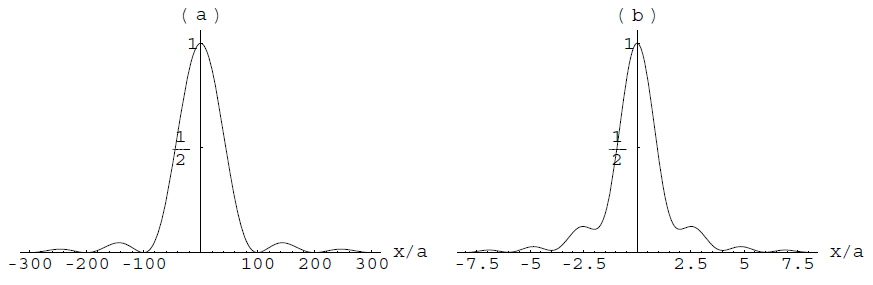
\includegraphics[width=13cm]{Imagenes/Fig9}
\caption[Patron de interferencia, 1 rendija, regimen de Fraunhofer]{Curva de difracción para una sola rendija, en la figura (a) $N_F(a)=0.01$, en (b) $N_F(a)=0.5$. Tomado de [1]}
\end{figure}
Sin embargo para $N_F(a)\ll 1$, obtenemos diferentes aproximaciones asintóticas:
\begin{eqnarray}
\nonumber &P^{(\text{1rendija})}(x)\simeq\frac{\gamma}{\eta}\left(\frac{\sqrt{N_{F}(a)}}{2a}+\frac{\text{\text{Sin}}\left(\frac{\pi}{2}N_{F}(a)\eta\left(1-\frac{x}{a\eta}\right)^{2}\right)}{2\pi\sqrt{\eta}\left(a-\frac{x}{\eta}\right)}+\frac{\text{\text{Sin}}\left(\frac{\pi}{2}N_{F}(a)\eta\left(1+\frac{x}{a\eta}\right)^{2}\right)}{2\pi\sqrt{\eta}\left(a+\frac{x}{\eta}\right)}\right)^{2}\\
&+\frac{\gamma}{\eta}\left(\frac{\sqrt{N_{F}(a)}}{2a}-\frac{\text{\text{Cos}}\left(\frac{\pi}{2}N_{F}(a)\eta\left(1-\frac{x}{a\eta}\right)^{2}\right)}{2\pi\sqrt{\eta}\left(a-\frac{x}{\eta}\right)}-\frac{\text{\text{Cos}}\left(\frac{\pi}{2}N_{F}(a)\eta\left(1+\frac{x}{a\eta}\right)^{2}\right)}{2\pi\sqrt{\eta}\left(a+\frac{x}{\eta}\right)}\right)^{2},|x|<a\eta
\end{eqnarray}
\begin{equation}
P^{(\text{1rendija})}(x,a)\simeq\frac{2\gamma}{\pi^{2}\eta^{2}}\left(\frac{a^{2}}{\left(\frac{x^{2}}{\eta^{2}}-a^{2}\right)^{2}}+\frac{1}{\left(\frac{x^{2}}{\eta^{2}}-a^{2}\right)}\text{Sin}^{2}\left(\pi N_{F}(a)\frac{x}{a}\right)\right), |x|>a\eta
\end{equation}
Esto se debe a que las aproximaciones asintóticas tienen el siguiente comportamiento:
\begin{eqnarray}
&\alpha(x,\pm a)\gg 1,\hspace{0.2cm} \text{si}\hspace{0.2cm} N_F(a)\gg 1 \hspace{0.2cm} \text{y}\hspace{0.2cm} |x|<a\eta\\
&\pm\alpha(x,\mp a)\gg 1,\hspace{0.2cm} \text{si}\hspace{0.2cm} N_F(a)\gg 1 \hspace{0.2cm} \text{y}\hspace{0.2cm} |x|>a\eta
\end{eqnarray}
La función (2.83) oscila rápidamente alrededor del valor constante $N_F(a)\gamma/2a^2\eta=1/(\lambda_z(L+D))$ en $|x|<a\eta$ y la función (2.84) decrece rapidamente a 0 en $|x|>a\eta$. La curva de difracción se muestra en la figura 2.10.
\begin{figure}[h]
\centering
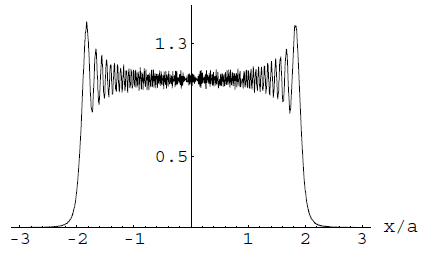
\includegraphics[width=10cm]{Imagenes/Fig10}
\caption[Patron de interferencia, 1 rendija, regimen de Fressnel]{Curva de difracción para una sola rendija, en la figura  $N_F(a)=100$. Tomado de [1]}
\end{figure}

\subsection{Interferencia y difracción por dos rendijas.}


\section{Campos escalares.}
\section{Campos fermiónicos.}
\section{Teorías Gauge y campos de Yang-Mills}
\section{La teoria de Yukawa}